\chapter{Changing control parameters}

With our new understanding of the normal operation and the meaning of dimensionless numbers, it makes sense to investigate how these behave when tweaking the turbine parameters. Plotting $C_P$ and $C_T$ as a function of the yaw and pitch-angle should hopefully give an intuition of how they affect power and loads in further analysis. Power and load are, of course, also dependent on rotational speed, so two contour plots are created to visualise this 4-dimensional space. 

\section{Dimensionless power}
\label{dimensionless_power}

Starting by exploring how yaw and pitch affect CP, the appropriate plot is illustrated in figure \ref{fig:cpcontour}.

\begin{figure}[H]
    \centering
    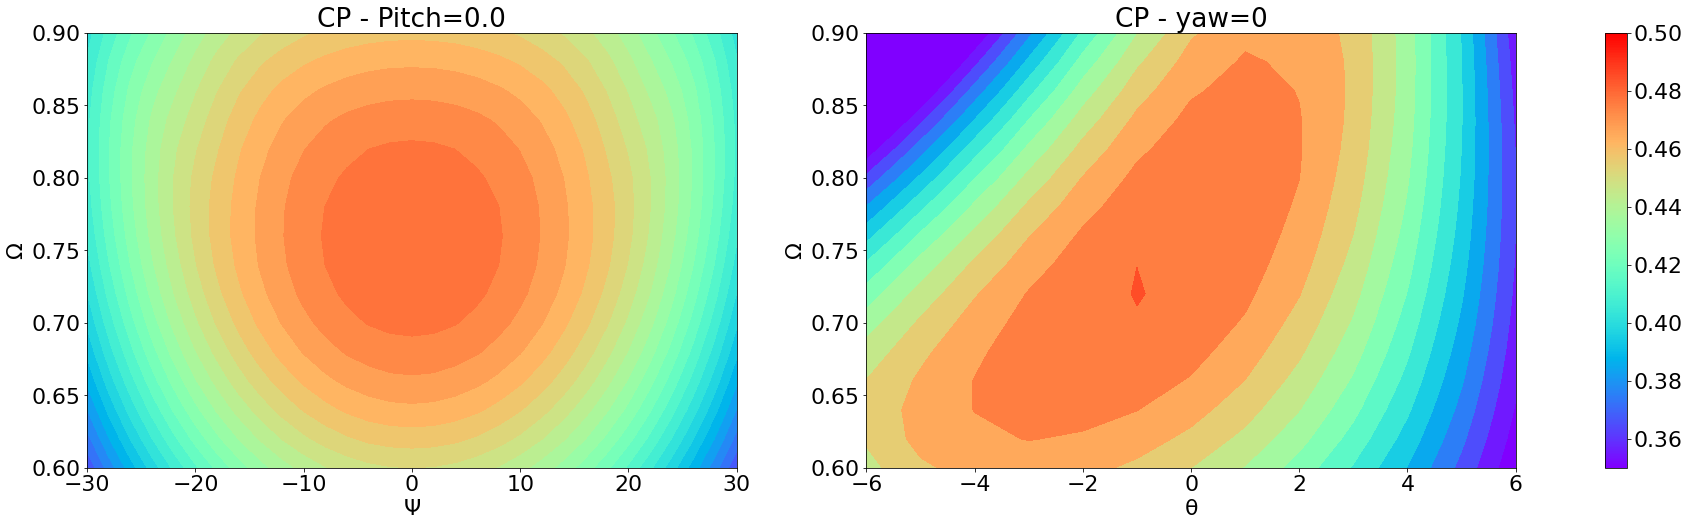
\includegraphics[scale=0.23]{Illustrations/cpcontour.png}
    \caption{$C_P$ as a function of $\Omega, \psi, \theta$ for $U=8 m/s$}
    \label{fig:cpcontour}
\end{figure}

What is immediately apparent is that the direction of the yawing does not seem to have any significant effect on the turbine within a reasonable range. Though this might be expected, it is not necessarily given, and it is pleasant to see the simulations backing up our intuition. Additionally, the turbine is most effective, operating at approximately $0.75 rad/s$, which matches the normal operation seen in figure \ref{fig:rotpitch}. For pitching, the optimal angle seems dependent on the rotational speed and appears negative for low rotational speeds and positive for high rotational speeds. However, similar to the yawing, this dependency is not very sensitive. We will therefore conclude that it is possible to both yaw and pitch to a certain degree without sacrificing any notable power. However, when reaching high angles, both seem to suffer significantly, which we should keep in mind for further analysis.

\section{Dimensionless thrust}

To do a similar analysis for CT, a matching plot is illustrated in figure \ref{fig:ctcontour}

\label{dimensionless_thrust}
\begin{figure}[H]
    \centering
    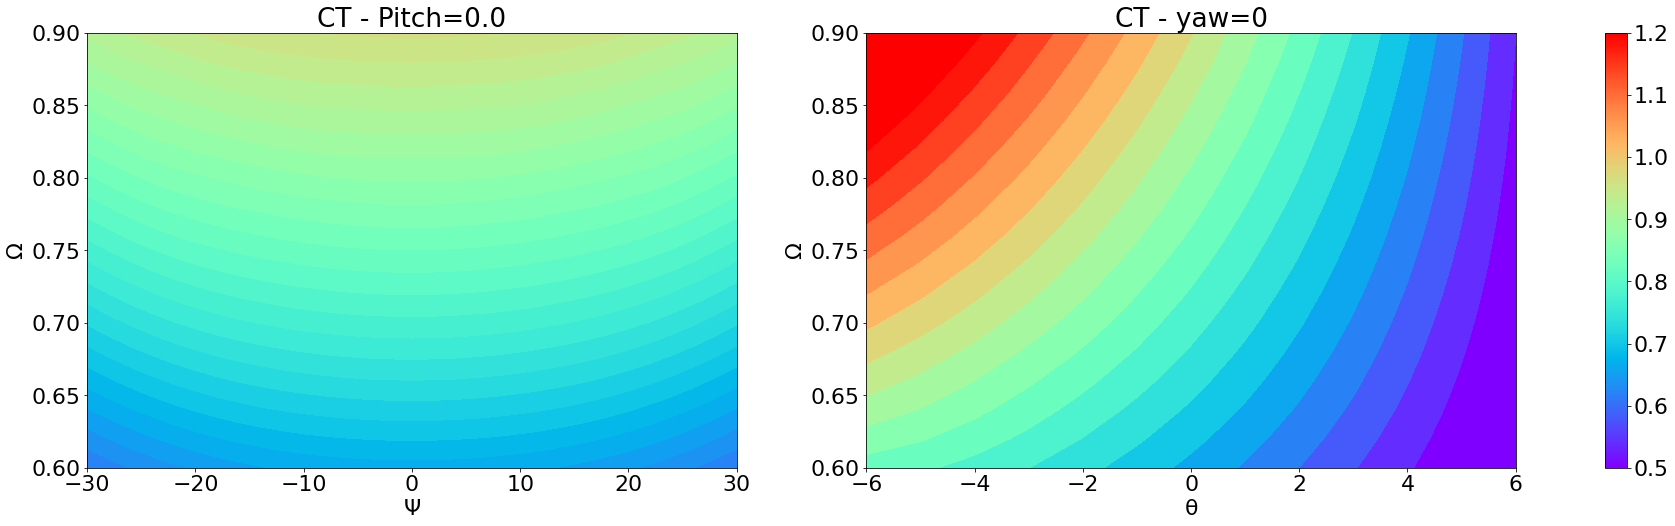
\includegraphics[scale=0.23]{Illustrations/ctcontour.png}
    \caption{$C_T$ as a function of $\Omega, \psi, \theta$ for $U=8 m/s$}
    \label{fig:ctcontour}
\end{figure}

Looking at $C_T$ as a function of yaw and rotational speed, we again see that the yawing direction does not seem to have any effect, just like we concluded for CP. What is, however, notable is that CT slightly decreases with larger angles. Though this is technically an advantage, we should remember from figure \ref{fig:cpcontour} that it also reduces power. For pitching, we see a similar trend for positive angles, as this also follows CP. However, negative angles induce much higher thrust while simultaneously producing less power. As one might expect, this is very unfavourable, and large negative pitching angles are, therefore, less interesting for further analysis.